\section{The expedition starts with a bang!}
The ICU Union minibus hauled itself into \passage{Tolmin} at midday on Saturday 8th July, as the thermometer rocketed through 30 degrees. Myself and Ben, who had come out a day early, drove our stolen shopping trolley, loaded with bread, sausage, iced-tea and booze. We converged with perfect timing at the old Jugoslav barracks, now the industrial estate, where one of our JSPDT friends has an injection-moulding factory. 

This was to be expedition base camp, the rack of toilets and cold water showers a perfectly match. After pizza, the van was partially unloaded into a more mountain-road friendly configuration. The smelly van-people headed off to the \passage{Soča} river (10 degrees, but very clean, at least upstream of cavers) to swim and sun worship. 

\begin{marginfigure}
\checkoddpage \ifoddpage \forcerectofloat \else \forceversofloat \fi
\centering
\frame{\includegraphics[width=\textwidth]{"images/2017/welcome-2017/matrjal_bajta_kau_2016__3_".jpg}}
\caption{The famous petrol motorbike was once again put to good use. Antonio of the JSPDT ferried most of the rigging gear from \protect\passage{Ravne} to \protect\passage{Kal} in an afternoon --- Jana \v{C}arga}
\label{motorbike}
\end{marginfigure}

\begin{marginfigure}
\checkoddpage \ifoddpage \forcerectofloat \else \forceversofloat \fi
\centering
\frame{\includegraphics[width=\textwidth]{"images/2017/welcome-2017/fratnik_in_helicopter".jpg}}
\caption{Other food supplies were helicoptered to \protect\passage{Kal} thanks to the Slovenian airforce, these included several kg of pasta, potatoes and onions --- Jana \v{C}arga}
\label{helicopter fratnik}
\end{marginfigure}

A crack(ed) team headed off to \passage{Tolminske Ravne} (at 925 m, the trail head). There are something like 30 hair-pin bends on the single track road from \passage{Tolmin}. Rather disturbingly, about half-way up, the van started belching  grey smoke out the side of the bonnet every time we braked. Not wanting to risk being stranded and blocking the single-track road halfway up, we limped our way into \passage{Ravne}. 

Rather than our standard parking spot next to a barn recently filled with ~50 cubic metres of wood for winter, we parked on the road surrounded by only concrete. Tentatively approaching the still smoking bonnet with fire-extinguisher in hand, we quickly located the fault. The cap to the coolant had been `repaired' with tinfoil and rubber bands, which had evidently fallen off at some point in the prior 1000 miles across Europe. The thirsty Transit drank 8 L of the best mountain water, and with a rather more heavy-duty cap improvisation constructed from a cave oversuit patch and a cable tie, was ready for more action. We unloaded the minibus. One driver drove back to \passage{Tolmin} to save the rest of the team from the fleshpots. 

\begin{figure*}[t!]
\checkoddpage \ifoddpage \forcerectofloat \else \forceversofloat \fi
\centering
    \begin{subfigure}[t]{0.413\textwidth}
        \centering
        \frame{\includegraphics[width=\linewidth]{"images/2017/welcome-2017/ben_crates".jpg}} 
        \caption{} \label{ben with crates}
    \end{subfigure}
        \hfill
\begin{subfigure}[t]{0.577\textwidth}
\centering
\frame{\includegraphics[width=\linewidth]{"images/2017/welcome-2017/solarpanel".jpg}}
 \caption{}\label{solar panels}
\end{subfigure}
\vfill
\begin{subfigure}[t]{\textwidth}
\centering
\frame{\includegraphics[width=\linewidth]{"images/2017/welcome-2017/full_barrell".jpg}}
 \caption{}\label{full barrel}
\end{subfigure}
  \caption{
    \emph{(a)} The 16 green crates ferried by minibus contain the bulk of our metalwork, rope and food supplies for a four week expedition --- Jarvist Frost
     \emph{(b)}  Solar power harnessed with two surface solar panels --- Tanguy Racine
     \emph{(c)}  A violent thunderstorm is enough to fill the four barrels and provide two weeks' worth of water supply for the expedition ---  Rhys Tyers}
\end{figure*}


Expo logistics revolve around the `green crates', 60 L packing crates of which we can stack 18 in the back of the 9 seater minibus. This enables us to start tooling up months before the expedition leaves, duck-taped labelled crates marching around our caving stores as drills are fettled and items arrive from various corners of the country and the internet. 

Somehow such ideals of organisation are never quite realised, and so sorting, relabelling, finding and prioritising objects for carrying up the hill took up the rest of the day. The whole team united at \passage[hamlet]{Ravne}, we took an early night, lined up on the floor of the little community common room made available for us this year. 

An extreme storm started at around 10 PM. The rain was so heavy and so driven that it slipped under the door, forming a 3 m diameter lake (sleeping bags evacuated by Tikka light), before slinking off into the toilet and disappearing down a drain.

Everyone was up at dawn, keen to avoid the heat of the climb. Most people were heading up the hill at 6, and so by 10 the plateau (~1850 m) was already dotted with tents. We spent Sunday in the Bivi. This is where we store gear and food in large Daren drums and 200 L blue plastic barrels over the winter. Our advanced party had unpacked these barrels, and setup our Tarpaulins which serve both to shelter the cooking and sitting area, and channel drinking water into the barrels. In spite of no one being present to tune the guy lines, we had a good few hundred litres of water already gathered. This we we spent during the day on scrubbing and sterilising the pots, pans, containers and gear which we had left up over the winter. 

\begin{figure*}[t!]
\checkoddpage \ifoddpage \forcerectofloat \else \forceversofloat \fi
\begin{subfigure}{0.975\textwidth}
\begin{tikzpicture}
\node [name-dest] (box){%
    \begin{minipage}{\textwidth}
    \begin{multicols}{2}
    Back up at the bivi after a beautiful day down from \passage{Ravne} to the \passage{Zadla\v{z}cica} – the water was quite refreshing, the current rather forgiving so a pause by a plunge pool at around midday inevitably ended with a bath. I am quite amazed at the coincidence which brought Tim, the German geologist to \passage{Ravne}. He met with Janet, explaining his plan to recce geological locations for a fieldtrip. We therefore set off together from the plateau, stopping here and there, chatting and taking in the geology along the \passage{Ravne}-\passage{Tolmin} switch back road. After taking plenty of notes at the outcrops of the \passage{Slovenska Geološka Pot} (Slovene geological path), getting lower and lower until midday.

    At the bridge, next to the hydro plant, the air was so hot we climbed down to the river level, hopping along the inclined bedding. Blue water sinking past us, goats on the other bank, what was not to like about this little spot of paradise?

    We stripped down and went in the deep pools, taking photos and cooling down. It was perfect. The only downside was the walk back to Ravne, during which all our efforts to stay dry, fresh and non-sweaty failed miserably. Back at \passage{Ravne} I ate most of the “Apéritif” crackers (Smoki’s), drank tea (courtesy of Ben) and took a karimat out to lie down in the shade. By 4:45pm, we were raring to go and started the long ascent to the Bivi. There awaited the best surprise of the day: food, though Antonio's sweet apricot schnapps came a close second.

    \begin{quote}I undersigned Tanguy Racine, self-respecting cook and amateur gastronome declare my papillae ‘blown away’ by the onion soup and chips which were left for us to eat.\end{quote} \name{Tanguy Racine}
      \end{multicols}
    \end{minipage}

};
\node[fancytitle, right=10pt] at (box.north west) {Escaping mountain `Clag'};
\end{tikzpicture}
\end{subfigure}
\par\bigskip
\begin{subfigure}{\linewidth}
\frame{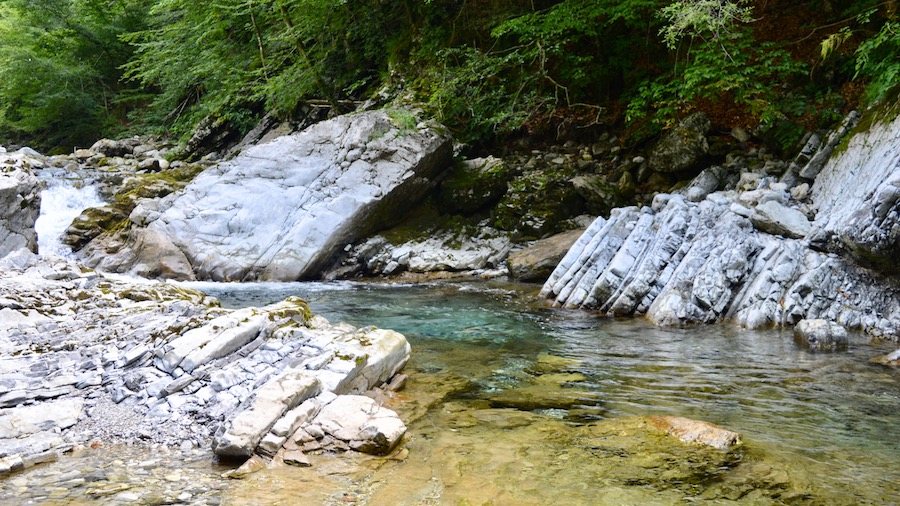
\includegraphics[width = \linewidth]{images/2017/welcome-2017/hydro river.jpg}}
\end{subfigure}
\caption[Zadla\v{z}cica]{The \protect\passage{Zadla\v{z}cica} river, just upstream of hydro-electrical station offers a profusion of sunlit riffles and pools --- Tanguy Racine}
\end{figure*}


The previous week a helicopter lift had been made by the Slovene cavers - bringing expedition essentials of petrol (to cook with), pasta, rice and cooking oil. It also brought luxuries. We marvelled at the string bags of potatoes and onions (fresh vegetables!). We also knew of the existence of 20 L of wine (a substance considered too lacking in proof to be worthy of a carry by human). This was then hidden, discovered, and re-hidden over the next few weeks, as various expedition members played the angels and devils of our collective conscience. 

More carries on Monday and Tuesday followed. We were mostly set up for caving, and teams had been to start the chin-scratching challenge of rigging the 150 m Abseil from the plateau to the cave entrance. This is problematic as it continuously varies from about 45 degrees to sheer. A vast quantity of scree is barely held back by scraggy grass and clumps of dwarf pine. Any scree knocked loose tended to bound its way down, making a terrifying `\emph{thrp-thrp-thrp}' as the uneven boulders tumbled their way to a terminal velocity. As well as this objective danger, the surface abseil was subjectively scary, being above the kilometre deep \passage[valley]{Polog} valley. 



Perhaps the worst situation was when the mountain was partly enveloped in cloud. It is very strange sensation to see a house appear through the fog a long way below, while at the same time a peak of the \passage[mountain]{Krn} massif winked at your from above. 

One problem was that we were already running low on water. Tuesday brought successively heavier rain storms. With frantic effort we tried to gather every drop, belaying the tarps by hand if necessary, siphoning water between barrels. \bignote{By 4 PM, it was clear that supply was going to outstrip storage no matter what we did, and we soon had four brim full barrels}, and replenished sealed 20 L containers of water. Perhaps 800 L in all - plenty for two weeks. 

\bignote{The weather did not get the message that we were sated, and redoubled its efforts}. Along with the incredibly heavily rain, there was an increasing cacophony of thunder and lightning. Cavers arrived in the Bivi from their carries with overflowing boots. By 8PM everyone was on the mountain, fed, watered and frankly bored. People sat around on the drier side of the stone circle, drinking tea in their waterproofs. 

The rain had lessened considerably, and the booming had moved off to the next set of peaks. Up on the plateau, rain was still falling, but it was pleasantly still. The occasional jagged line cut through the sky, touching the ridge many kilometres downwind. Tanguy dashed to his tent: `\textit{You can't outrun lightning!}' I shouted after him. Such japes! A recurrent strike hit a mountain not so far away, and at least 500 m below us. Troubling. Soon after there was a little strike on \passage{Migovec} itself, roughly our altitude and more importantly, upwind. It was time to return to the safety of the Bivi.

\begin{figure*}[t!]
\checkoddpage \ifoddpage \forcerectofloat \else \forceversofloat \fi
\centering
\frame{\includegraphics[width=\textwidth]{"images/2017/welcome-2017/lightning".jpg}}
\caption{Lightning often hits the plains of Italy, making for a beautiful display of light and shadows--- Arun Paul}
\label{lightning}
\end{figure*}


The event was not noise or light, but all at once.  Even the dark green dwarf pine was lit so bright it became white. It felt like I'd been hit very hard over the head with a cricket bat. This was replaced by a sense that my head and hair was on fire. Rubbing at the fire frantically, I was amazed to find all my greasy locks were still there. My hat was missing (magically to be found later in my pocket). My head was full of white noise, and horrible black puddles of amnesia. Had I hit the ground? How long had it been? I was staring at my tingling hands, amazed that they were there and functional. 

As my hearing returned, I could hear the screaming - multiple voices overlayed. It gave me something to focus on. I stepped up to the Bivi and gazed down on pandemonium. 

I knew lightning was involved, but my first thought was that the petrol lantern we use for evening light had exploded. The stone circle we sit around was empty, people having thrown themselves backwards and outwards. About half the occupants were walking wounded, a quarter writhing on the floor screaming and clutching legs, and a quarter ominously still and quiet. Everyone had been effected.

It was impressive to see the walking wounded stagger around with numbed legs, swallowing down the stress, calmly shouting over the thunder-clapped deafness, to follow their first aid training to assess, triage and treat. Everyone was confirmed as breathing. Casualty reports of burning legs showed no surface wounds. There was nothing we could think to do to deal with the reports of leg paralysis. So those unable to move we reassured, and bodily lifted out of the rain to place them back on the insulating carry mat of the stone circle. 

\margininbox{Log entries}{
It just came with a white glow and a deafening blow and the next moment I realised I was on the floor with both my legs feeling numb. -- \mininame{Larry Jiang}

\vspace{3mm}
There was a loud bang and my right leg exploded in pain. I flung myself back, and my left arm hit the rock. Everyone was screaming. \mininame{Jack Hare}

\vspace{3mm}
I'm alternating between an odd giddy joy, dumbstruck and vague existential dread. Struck by fucking lightning! Tick that one off the bucket list. -- \mininame{Rhys Tyers}

\vspace{3mm}
So, I found a four-leaf clover...\\
AND THEN WE GOT STRUCK BY LIGHTNING?\\
Felt like sleep paralysis.\mininame{Rebecca Diss}
}

We retreated into the driest corner of the Bivi, to wait out the lightning with fearful eyes. We sang songs and rubbed numb legs. After four hours, the lightning was long gone and we cautiously headed to bed. The two worst effected were still incapable of standing unaided. They were carried to bed between two helpers. Most people sleeping rejigged arrangements to acquire a tent fellow. The key question - how much of a Faraday cage do you reckon your tent is?

By the next morning, everyone could walk again. Some people (but not necessarily correlated with the worst effected) had amazing fern-like and starfish patterns burnt into their legs with burst capillaries. One person had an extensive pattern on their legs, and a matching mirror image in silver written in their black synthetic leggings. One expedition member left for London the next day, no longer feeling safe on the mountain top. The weather was thankfully thunder free for the next week, otherwise I suspect considerably more members would have left. 

The leg numbness slowly went away over a week, people were still staggering as their nerves slowly came back on line. Everyone seems to have made a complete recovery. Our cheap \textit{Survex} laptop did not work. One of our survey compasses (kept in a metal ammo box) had a +90 deg error. We can't be certain these were due to the lightning current, but we only discovered them after the strike.


\margininbox{More logbook extracts}{
We collected ourselves around the stone area, deeper in the bivi. There was some talking, mostly shocked and a bit shaken, trying to determine what had happened and who had been where and the damage done. Wine and Laško were passed round and we sang songs, which was a grateful distraction. -- \mininame{Celia Tinsley}

\vspace{3mm}
I have a lovely burn on my bum, and most of the damage isn't cellulite. -- \mininame{David Kirkpatrick}

\vspace{3mm}
`Where were you when the lightning struck the bivi?'\\
`In the bivi!' -- \mininame{Jack Hare}

\vspace{3mm}
\textit{Months later:} I still have mild tinnitus which started in one ear and is now affecting both, and seems unlikely to go away. -- \mininame{Dave Wilson}}


Perhaps unsurprisingly, the lightning strike definitely slowed down the rate at which we got properly underground.  The main effect was, of course, psychological. I certainly found it difficult to be planning trips with people I had just a couple of days previous been uncertain whether they were dead or alive. The beautiful plateau with its adders and rock falls, and the cave with its loose choss and uncertain rigging, took on a distinctly sinister air.

Nevertheless, by the end of the first week, the first newly explored survey data was coming back from the cave.

The mountain-top life continued much as it does in any other year. Ukulele and guitar lessons were given and received. Rewording of songs to give them a caving meaning an ever popular past-time. \sidenote{Leonard Cohen's `Hallelujah' a fitting favourite this year!} Experimental cooking took us to savoury doughnuts, filled with cheese. The helicoptered bags of potatoes were chipped and deep fried, the soft onions souped.
\name{Jarvist Frost}

\fullwidthbox{Hare Cave}{
Gosh, what a day! Overcome by ennui, I had to break free. Rhys agreed to accompany me to `Hare cave', last pushed in 2004 by Jarv and Ben Ogborne. It terminates in a dog-leg in a human-sized phreatic.
The clag was thick, the far side of every shakehole just a vague outline. 
We dropped down into it and I went through into a collapse chamber filled with debris.
After a bit of hammering in the rift I kindly sent Rhys first.
\name{Jack Hare}
\vspace{3mm}

Wiggling up was now significantly easier and I was quickly lying prone in the meander. 
One arm forward and one back I \emph{reptated} forward. The tube is exactly body sized and there are two body lengths before a dogleg that stopped the previous team. 
Bending my back round the first corner, my head cleared the second. 

The cave died in that moment. 

\name{Rhys Tyers}}


